\documentclass[12pt]{article}
\setlength{\oddsidemargin}{0.25 in}
\setlength{\evensidemargin}{-0.25 in}
\setlength{\topmargin}{-0.6 in}
\setlength{\textwidth}{6.5 in}
\setlength{\textheight}{8.5 in}
\setlength{\headsep}{0.75 in}
\setlength{\parindent}{0 in}
\setlength{\parskip}{0.1 in}

%
% ADD PACKAGES here:
%

\usepackage{amsmath,amsfonts,amssymb,graphicx,mathtools}
\usepackage{multirow,url}

%
% The following commands set up the lecnum (lecture number)
% counter and make various numbering schemes work relative
% to the lecture number.
%
\newcounter{lecnum}
\renewcommand{\thepage}{\thelecnum-\arabic{page}}
\renewcommand{\thesection}{\thelecnum.\arabic{section}}
\renewcommand{\theequation}{\thelecnum.\arabic{equation}}
\renewcommand{\thefigure}{\thelecnum.\arabic{figure}}
\renewcommand{\thetable}{\thelecnum.\arabic{table}}

%
% The following macro is used to generate the header.
%
\newcommand{\lecture}[4]{
   \pagestyle{myheadings}
   \thispagestyle{plain}
   \newpage
   \setcounter{lecnum}{#1}
   \setcounter{page}{1}
   \noindent
   \begin{center}
   	\framebox{
   		\vbox{\vspace{2mm}
   			\hbox to 6.28in { {\bf MATH 254: Introduction to Statistics
   					\hfill #3} }
   			\vspace{4mm}
   			\hbox to 6.28in { {\Large \hfill Lesson #1: #2  \hfill} }
   			\vspace{2mm}
   			\hbox to 6.28in { {\hfill Corresponding Workbook Module: #4} }
   			\vspace{2mm}}
   	}
   \end{center}
   \markboth{Handout #1}{Handout #1}

   %{\bf Note}: {\it LaTeX template courtesy of UC Berkeley EECS dept.}

   %{\bf Disclaimer}: {\it These notes have not been subjected to the usual scrutiny reserved for formal publications.  They may be distributed outside this class only with the permission of the instructor.}
   %\vspace*{4mm}
   \vspace*{-4mm}
}
%
% Convention for citations is authors' initials followed by the year.
% For example, to cite a paper by Leighton and Maggs you would type
% \cite{LM89}, and to cite a paper by Strassen you would type \cite{S69}.
% (To avoid bibliography problems, for now we redefine the \cite command.)
% Also commands that create a suitable format for the reference list.
\renewcommand{\cite}[1]{[#1]}
\def\beginrefs{\begin{list}%
        {[\arabic{equation}]}{\usecounter{equation}
         \setlength{\leftmargin}{2.0truecm}\setlength{\labelsep}{0.4truecm}%
         \setlength{\labelwidth}{1.6truecm}}}
\def\endrefs{\end{list}}
\def\bibentry#1{\item[\hbox{[#1]}]}

%Use this command for a figure; it puts a figure in wherever you want it.
%usage: \fig{NUMBER}{SPACE-IN-INCHES}{CAPTION}
\newcommand{\fig}[3]{
			\vspace{#2}
			\begin{center}
			Figure \thelecnum.#1:~#3
			\end{center}
	}
% Use these for theorems, lemmas, proofs, etc.
\newtheorem{example}{Example}[lecnum]
\newtheorem{exercise}{Exercise}[lecnum]

\newtheorem{theorem}{Theorem}[lecnum]
\newtheorem{definition}[theorem]{Definition}
\newenvironment{proof}{{\bf Proof:}}{\hfill\rule{2mm}{2mm}}

% **** IF YOU WANT TO DEFINE ADDITIONAL MACROS FOR YOURSELF, PUT THEM HERE:

\newcommand\E{\mathbb{E}}

\begin{document}
%FILL IN THE RIGHT INFO.
%\lecture{**LECTURE-NUMBER**}{**DATE**}{**LECTURER**}{**SCRIBE**}
\lecture{2}{Inference for a Population Mean}{Mintaek Lee}{3}
%\footnotetext{These notes are partially based on those of Nigel Mansell.}

% **** YOUR NOTES GO HERE:
\begin{example}
	Mintaek loves hamburgers. He regularly eats a Quarter Pounder\textsuperscript{\textregistered} with Cheese at the local McDonald's restaurant. Since Mintaek is particular about what he eats, he grows suspicious that the patties in the burger are actually less than 0.25 lbs. He randomly picks 51  McDonald's restaurants in the Pacific Northwest region and buys 1 Quarter Pounder\textsuperscript{\textregistered} with Cheese from each of them. He then weighs each patty using a reliable scale. His samples had a mean of 0.227 lbs and a standard deviation of 0.084. Does the evidence Mintaek collected support Mintaek's claim or not? Use the appropriate statistical procedure and hypotheses that best match Mintaek’s interests. Use a 0.05 level of significance.
\end{example}
	
\noindent \textbf{Step 1}: Note that the McDonald's claim is $H_0$ since Mintaek has not found any evidence against them yet, thus it is considered to be the status quo. The alternative hypothesis would be Mintaek's claim. Since Mintaek wanted to show that the average weight of patties is actually less than 0.25 lbs, the $H_A$ is $\mu < 0.25$.
\begin{itemize}
	\item $H_0$: $\mu = 0.25$, population mean weight of patties is equal to 0.25 lbs
	\item $H_A$: $\mu < 0.25$, population mean weight of patties is \textbf{less than} 0.25 lbs
\end{itemize}

\noindent \textbf{Step 2}: We first must acknowledge that the population standard deviation, $\sigma$, is unavailable to us and the sample size is not several hundreds ($n=51$). Thus we can't use the one-sample z-test and need to use the one-sample t-test. First, we check all the underlying conditions (See Workbook page 91 for the description of conditions). For the significance level, you may use $\alpha = 0.05$ which is an industry standard, unless otherwise specified.

We check the following conditions for the one-sample t-test for a mean:
\begin{itemize}
	\item The population standard deviation $\sigma$ is unavailable, so we must calculate the sample standard deviation $s$.
	\item Since $n = 51 > 40$, we can assume that we have a normal sampling distribution.
	\item Each observation can be assumed to be independent since Mintaek bought each burger from a randomly chosen restaurant.
	\item Population size ($N$) is certainly larger than 10 times the sample size ($n=51$). \\
	(McDonald's certainly has made more than 510 Quarter Pounders\textsuperscript{\textregistered} with Cheese.)
\end{itemize}
Since all conditions are met, we can use the one-sample t-test to make an inference on $\mu$, the population mean (the average weight of ALL burger patties, not just the 51 of them that Mintaek bought). Note again that the sample size is too small to use the one-sample z-test. We would need the sample size to be at least several hundreds to safely use the z-test when we do not have $\sigma$, the population standard deviation.

\noindent \textbf{Step 3}: We can now find the t-test statistic value and corresponding P-values. Recall that we are given $\bar{x} = 0.227$, $s = 0.084$, and $n=51$ from the question.

For $df = n - 1 = 51 - 1 = 50$, we obtain
\begin{align*}
t &= \dfrac{\bar{x} - \mu_0}{s / \sqrt{n}} 
= \dfrac{0.227 - 0.25}{0.084 / \sqrt{51}}
= \dfrac{-0.023}{0.011762}
= -1.9554
\end{align*}
where $\mu_0$ is the hypothesized population mean from the hypotheses.

At the t-distribution table, look at the row corresponding to $df = 50$. We can see that the positive value of our t-test statistic $t = 1.9554$ is between 1.676 and 2.009. Note that I am using the positive value of $t$ because t-distribution is symmetric. It means the tail area to the right of $t = 1.9554$ (lower tail area) is going to be the same as the tail area to the left of $t = -1.9554$ (upper tail area). In this context, area = proportion = probability.

Since the upper tail probability $p$ corresponding to $t = 1.676$ and $t = 2.009$ are 0.05 and 0.025, respectively, we can guess that the \textbf{upper} tail probability $p$ corresponding to our t-test statistic $t = 1.9554$ is between 0.05 and 0.025. Therefore, the \textbf{lower} tail probability $p$ corresponding to our t-test statistic $t = -1.9554$ is between 0.05 and 0.025.

We are only interested in the lower tail since we only care about checking if the $\mu$ is less than 0.25 or not. So we do not consider the upper tail area. Therefore, our P-value would be just $0.025 <$ P-value $< 0.05$.

\noindent \textbf{Step 4}: Our P-value was less than $\alpha = 0.05$. So we would reject the null hypothesis that population mean weight of patties is less than 0.25 lbs with the significance level of $\alpha = 0.05$. 

It means that we have sufficient evidence to suggest that the mean weight of patties of ALL Quarter Pounders\textsuperscript{\textregistered} with Cheese sold by McDonald's in the Pacific Northwest region is less than 0.25 lbs.

\vspace{10 pt}

\textbf{\textit{IF THIS WAS A TWO-SIDED TEST WHERE $\boldsymbol{H_A}$: $\boldsymbol{\mu \neq 0.25}$}}

\vspace{10 pt}

\noindent \textbf{Step 1}: $H_0$ is the same. Just $H_A$ needs to be changed.
\begin{itemize}
	\item $H_0$: $\mu = 0.25$, population mean weight of patties is equal to 0.25 lbs
	\item $H_A$: $\mu \neq 0.25$, population mean weight of patties is \textbf{not equal to} 0.25 lbs
\end{itemize}

\noindent \textbf{Step 2}: Same.

\noindent \textbf{Step 3}: This would be a two-sided test. It means that we are interested in both tails of the sampling distributions. In other words, we are interested in seeing if population mean weight of patties ($\mu$) is much higher than 0.25 or much lower than 0.25. So we need to combine the lower tail probability and upper tail probability (or simply double the lower tail probability, since they will be equal) to cover the areas of both tails.

Remember that in earlier we found that the \textbf{upper} tail probability $p$ corresponding to our t-test statistic $t = 1.9554$ is between 0.05 and 0.025, and the \textbf{lower} tail probability $p$ corresponding to our t-test statistic $t = -1.9554$ is between 0.05 and 0.025.

Therefore, our P-value would be between $2 \times 0.05$ and $2 \times 0.025$, that is 0.1 and 0.05. We can express our P-value as: $0.05 <$ P-value $< 0.1$.

\noindent \textbf{Step 4}: Our P-value was greater than $\alpha = 0.05$. So we would fail to reject the null hypothesis that population mean weight of patties is not equal to (or different from) 0.25 lbs with the significance level of $\alpha = 0.05$. 

It means that we do not have sufficient evidence to suggest that the mean weight of patties of ALL Quarter Pounders\textsuperscript{\textregistered} with Cheese sold by McDonald's in the Pacific Northwest region is different from 0.25 lbs.

Notice that we got a different conclusion than the earlier one-sided test case. It is important to set up your hypotheses accordingly to best match your interests.

\vspace{20 pt}

\textbf{On Checking Conditions}:
\begin{itemize}
	\item There are 3 ways to meet the ``normal sampling distribution'' condition for the one sample t-test (second condition under step 2 in workbook page 91).
	\begin{itemize}
		\item If $n \geq 40$, you are good to go. No need to graph anything.
		\item If $16 \leq n < 40$, you need to make a histogram of your samples to make sure that it is not too skewed or has no outliers. It does not have to look perfectly symmetric.
		\item If $n < 16$, you need to make a histogram of your samples to make sure that the sample could have come from a normal population. It will need to be fairly symmetric and have no outliers.
	\end{itemize}
	\item There are 2 ways to meet the ``normal sampling distribution'' condition for the one sample z-test (second condition under step 2 in workbook page 82).
	\begin{itemize}
		\item If $n \geq 30$, you are good to go. No need to graph anything.
		\item If $n < 30$, you need to make a histogram of your samples to make sure that the sample could have come from a normal population. It will need to be fairly symmetric and have no outliers.
	\end{itemize}
\end{itemize}

\pagebreak

\begin{example}
	Mintaek now wants to estimate what really is the population mean weight of patties of Quarter Pounders\textsuperscript{\textregistered} with Cheese. So he decides to make a 95\% confidence interval.
\end{example}
	
\noindent \textbf{Step 1}: Technically, you still would need to check all conditions for t-confidence intervals. However, you may notice that they are identical to ones for the t-test. So, you could omit this section if you already answered the Question 1.

We check the following conditions for the one-sample t-confidence interval for a mean:
\vspace{-5pt}
\begin{itemize}
	\item The population standard deviation $\sigma$ is unavailable, so we must calculate the sample standard deviation $s$.
	\item Since $n = 51 > 40$, we have a normal sampling distribution.
	\item Each observation is independent since Mintaek bought each burger from a randomly chosen restaurant.
	\item Population size ($N$) is certainly larger than 10 times the sample size ($n=51$).
\end{itemize}
Since all conditions are met, we can use the one-sample t-confidence interval to make an inference on $\mu$. Note that the sample size is too small to use one-sample z-confidence interval. We would need our sample size to be at least several hundreds to safely trust the z-confidence interval when we do not have $\sigma$ given to us.

\noindent \textbf{Step 2}: We first need to calculate the margin of error in order to construct the appropriate t-confidence interval. The margin of error is
\begin{align*}
m &= t^* \dfrac{s}{\sqrt{n}}
\end{align*}
for $df = n-1 = 51 - 1 = 50$.

Since we have $s = 0.084$ and $n = 51$ given from the question, we only need to find $t^*$. Notice that $t^*$ is different from $t$ from Question 1. $t^*$ here is called the t-critical value and you find it from the t-distribution table using appropriate $df$ and confidence level.

We want to construct 95\% confidence interval and have $df = 51 - 1 = 50$. So we look at the row corresponding to $df = 50$ on the t-distribution table. We then find a column corresponding to the confidence level 95\% from the last row. We should find $t^* = 2.009$ as appropriate critical value.

We can then find the margin of error as
\begin{align*}
m &= t^* \dfrac{s}{\sqrt{n}} 
= 2.009 \times \dfrac{0.084}{\sqrt{51}}
= 0.0236
\end{align*}

\noindent \textbf{Step 3}: We can now construct the 95\% confidence interval for $\mu$, population mean weight of patties. Remember that $\bar{x} = 0.227$.
\begin{align*}
\bar{x} \pm m = 0.227 \pm 0.0236 = (0.227 - 0.0236, 0.227 + 0.0236) = (0.203, 0.251)
\end{align*}

This means that we are 95\% certain/sure/confident that the interval (0.203, 0.251) would contain $\mu$, mean weight of patties of ALL Quarter Pounders\textsuperscript{\textregistered} with Cheese sold by McDonald's in the Pacific Northwest region.

%\pagebreak
\vspace{20 pt}

\textbf{When do I use $\boldsymbol{t}$ or $\boldsymbol{z}$?}:
\begin{itemize}
	\item $t$ and $z$ serve the same purpose. They just have different requirements to be used.
	\item If the population standard deviation $\sigma$ is given to you and/or the sample size is at least couple hundreds, you should use the one-sample z-test for a mean or one-sample z-confidence interval for a mean.
	\item If the population standard deviation $\sigma$ is NOT given to you (so you had to calculate the sample standard deviation $s$) and the sample size is NOT couple hundreds, you should use the one-sample t-test for a mean or one-sample t-confidence interval for a mean.
\end{itemize}

\textbf{Additional Practice Suggestions}:
\begin{itemize}
	\item Note that if we had much larger sample size, such as, $n = 500$, (or had the population standard deviation $\sigma$ given) we would have been able to use the one-sample z-test for a mean for Question 1 and one-sample z-confidence interval for a mean for Question 2.
	\item For Question 1, you would instead calculate z-test statistic $z$ and find appropriate tail areas using the standard normal distribution (z) table.
	\item For Question 2, you would instead find the z-critical value which you can find at the last row of the t-distribution table.
	\item Also note that conditions you need to check for z-test and z-confidence interval are slightly different from t-test and t-confidence interval, respectively. See workbook page 62 for conditions.
	\item It would be a good exercise to work through this example twice.
	\begin{itemize}
		\item First, change the sample size to $n = 300$ from $n = 51$ and repeat the example problem accordingly.
		\item Second, change the question so that you are given the population standard deviation of weights of patties as $\sigma = 0.084$ (leave $n$ as 51) and repeat the example problem accordingly.
	\end{itemize}
\end{itemize}


\pagebreak

\textbf{How to calculate exact P-values using software}:

In this handout, we used the $t$-distribution table to best approximate our P-values. For some homework problems and mini projects, you will need to find exact P-values. Although you will need to use your table to approximate your P-values on the exams. Here, I will demonstrate on how to find exact P-values using software.

I recommend this website: \url{https://surfstat.anu.edu.au/surfstat-home/tables/t.php}

\begin{figure}[!h]
	\centering
	\vspace{-10 pt}
	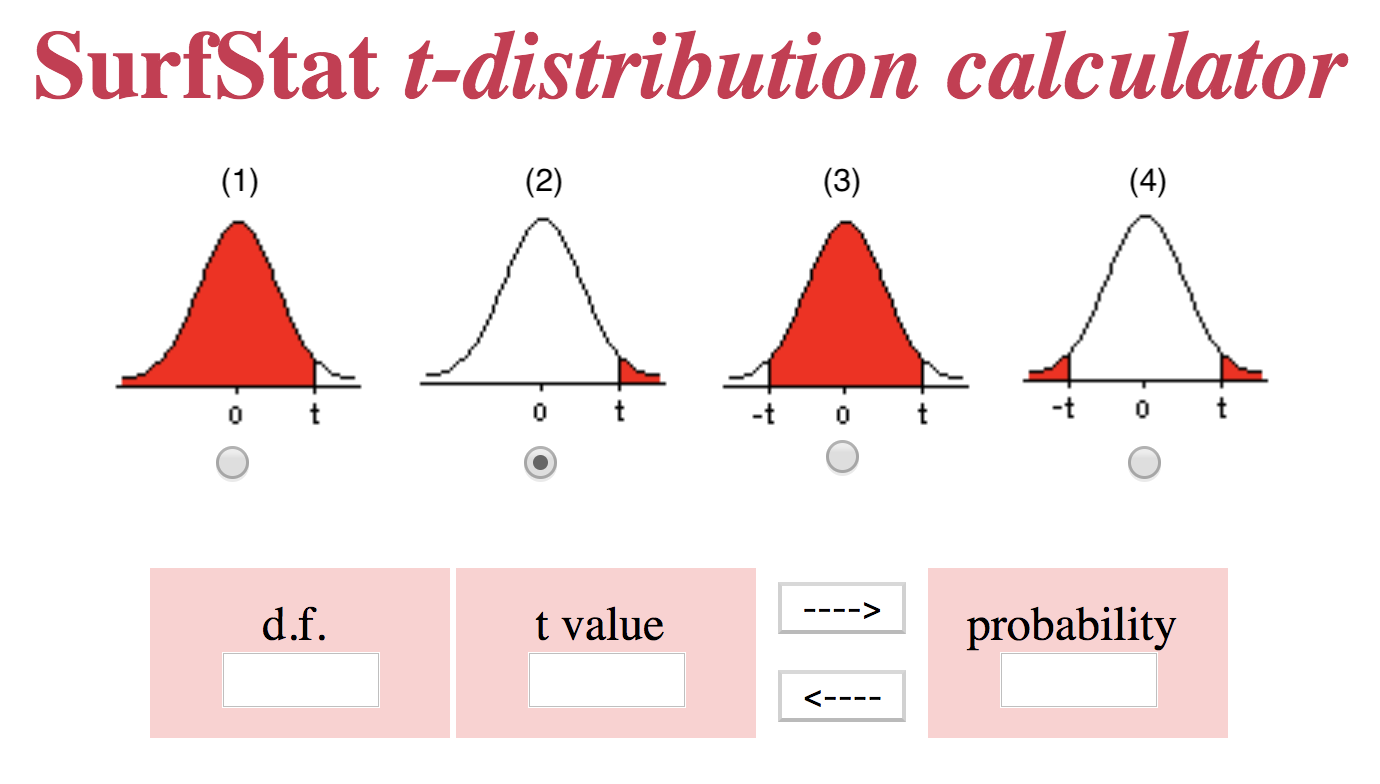
\includegraphics[width=12cm]{Figures/fig13.png}
	\vspace{-10 pt}
\end{figure}

You have four graphs to choose from in the website. I added numbers (1) -- (4) on top of each option for explanation purposes.
\begin{itemize}
	\item Select option (1) for the one-sided test that has the `$<$' sign in your $H_A$.
	\item Select option (2) for the one-sided test that has the `$>$' sign in your $H_A$.
	\item Select option (3) to get the $t$ critical value for confidence intervals.
	\item Select option (4) for the two-sided test that has the `$\neq$' sign in your $H_A$.
\end{itemize}

For (1), (2), and (4), enter your df (degrees of freedom) under `\textit{d.f.}' and $t$-test statistic under `\textit{t value}', then click `- - - -$>$' button to get the P-value which will appear under `\textit{probability}'.

For (3), enter your df (degrees of freedom) under `\textit{d.f.}' and desired confidence level under `\textit{probability}' (make sure to enter it in a probability format, i.e. a number between 0 and 1), then click `$<$- - - -' button to get the $t$ critical value which will appear under `\textit{t value}'.

\end{document}